\documentclass[12pt]{article}
\usepackage[margin=1.0in]{geometry}
\usepackage{amsmath}
\usepackage{amsfonts}
\usepackage{graphicx}

\newcommand{\N}{\mathbb{N}}
\newcommand{\Z}{\mathbb{Z}}
\newcommand{\Q}{\mathbb{Q}}
\newcommand{\R}{\mathbb{R}}
\newcommand{\C}{\mathbb{C}}

\newcommand{\norm}[1]{\left\lVert#1\right\rVert}
\newcommand{\ceil}[1]{\lceil#1\rceil}
\newcommand{\ov}{\overline}
\newcommand{\cleq}{\preccurlyeq}
\newcommand{\cgeq}{\succcurlyeq}
\newcommand{\bdy}{\textbf{\text{Bdy}}}
\newcommand{\trace}{\text{trace}}
\newcommand{\dom}{\textbf{dom}}
\newcommand{\expec}{\mathbb{E}}
\newcommand{\bigO}{\mathcal{O}}
\newcommand{\tr}{\text{tr}}
\newcommand{\<}{\langle}
\renewcommand{\>}{\rangle}

\usepackage[dvipsnames]{xcolor}
\usepackage{xspace}
\usepackage{url,comment,bm}

% \usepackage{titlesec}
% \setcounter{secnumdepth}{4}
% \titleformat{\paragraph}
% {\normalfont\normalsize\bfseries}{\theparagraph}{1em}{}
% \titlespacing*{\paragraph}
% {0pt}{3.25ex plus 1ex minus .2ex}{1.5ex plus .2ex}

% please pick visible and different from others colours - see list at the end of the page https://www.overleaf.com/learn/latex/Using_colours_in_LaTeX
\newcommand{\misha}[1]{{\color{Maroon} Misha says: #1\xspace}}

\newcommand{\todo}[1]{{\color{Red} TODO: #1\xspace}}


\title{Velocity gradient prediction using parameterized Lagrangian deformation models}

\author{Criston Hyett, Yifeng Tian, Michael Woodward, Misha Stepanov,\\ Chris Fryer, Michael Chertkov, Daniel Livescu}

\graphicspath{{./figs/}}
\begin{document}
\maketitle
\abstract{
We seek to efficiently predict the statistical evolution of the velocity gradient tensor (VGT) by creating local models for the pressure Hessian. Previous work has identified physics-informed machine learning (PIML) to be adept in this prediction; of note in this class of models is the Tensor Basis Neural Network (TBNN) for its embedded physical constraints and demonstrated performance. Simultaneously, phenomenological models were advanced by approximating the local closure to the pressure Hessian via deformation models using the history of the VGT. The latest in this series of models is the Recent Deformation of Gaussian Fields (RDGF) model. In this work, we combine the (local in time) PIML approach with the phenomenological idea of Lagrangian deformation to create a data-driven Lagrangian deformation model. We compare the model performance to both the TBNN and the RDGF models, and provide data-driven hypotheses regarding the Lagrangian upstream assumptions made in the RDGF model.

}

\section{Introduction} \label{sec:intro}

% The Lagrangian velocity gradient tensor (VGT) is a fundamental quantity in turbulence. 
% It displays characteristic non-Gaussian statistics (e.g., intermittency), describes the deformation rate of a fluid volume, and encapsulates alignment between strain and vorticity \cite{meneveau2011lagrangian}.
% % connect fundamental nature of VGT to its role in turbulence models
% Creating reduced-order models for the evolution of the VGT increases the fidelity of smallest-scale closures in e.g. LES \cite{needed}.

% % Make the negative statement "too expensive to directly compute" and motivate the need for ROMs
% Despite ever-growing computation capability, direct numerical simulation (DNS) of Navier-Stokes is still prohibitively expensive for realistic Reynolds numbers.


% % Now introduce the family of ROMs

% % Since the pioneering work of Viellefosse \cite{viellefosse1982} and the study of Cantwell\cite{cantwell1990} that showed that no exact local model exists for the evolution of the VGT, closure models for the VGT have received considerable attention;
% Since the pioneering work of Viellefosse \cite{viellefosse1982}, the VGT has received considerable attention; reinvigorated recently by enormous datasets generated via DNS.
% Machine learning (ML), specifically physics-informed machine learning (PIML), has shown remarkable ability to glean predictive capability from these large datasets, suggesting that unexploited patterns exist in the physics that we are still unaware of.

% % ----- rewrite progress -----
% Of particular note in recent years is the Recent Deformation of Gaussian Fields model (RDGF) \cite{johnson2016}, wherein the authors postulate a closure of the VGT evolution equations via choosing a Gaussian upstream condition that is deformed according to the current VGT. This hypothesis is in the same spirit as the Tetrad model from Chertkov et.al \cite{chertkov1999} that proposed a local closure to the VGT equations, by closing the equations for the VGT using deformation of a small fluid element. 

% In the realm of machine learning, this work is inspired by Tian et.al\cite{tian2021}, that used a highly structured, so-called Tensor Basis Neural Network (TBNN) architecture to close the equations. This network structure was inspired by theoretical work by \cite{pope1975}, \cite{lawson2015}, \cite{johnson2016}. It has been shown to explicitly respect Galilean and rotational invariance, enforce incompressibility, and after training, can predict many quantities of interest in the statistics of the VGT.

% Our goals in this paper are to advance the phenomenology via data analysis, and leverage this to improve the TBNN methodology to better predict the statistical evolution of the VGT.


The Lagrangian velocity gradient tensor (VGT) captures many fundamental aspects of turbulence; it displays non-Gaussian statistics (e.g., intermittency) including those of energy dissipation, describes the deformation rate of a fluid volume, and encapsulates alignment between strain and vorticity.
Because of its fundamental nature, understanding the evolution of the VGT is central to modern turbulent modeling challenges. E.g., creating better sub-grid models in LES\cite{silvis2017}.
However, despite ever-growing computation capability, resolving the VGT using direct numerical simulation (DNS) of Navier-Stokes is still prohibitively expensive for realistic Reynolds numbers.

Initiated by the work of Viellefosse, who examined keeping only the purely local contribution to the VGT evolution, "local closures" for the evolution of the VGT have recieved considerable attention. Viellefosse and subsequent work from Cantwell showed a finite time singularity originating from this so-called Restricted Euler dynamics. Further development in these local closures worked to resolve this finite time singularity; e.g., stochastic diffusion model\cite{girimaji1990diffusion}, linear damping model \cite{martin1998dynamics}, tetrad model \cite{chertkov1999}, linear diffusion model\cite{jeong2003velocity}, recent fluid deformation approximation \cite{chevillard2006lagrangian}, among others\cite{meneveau2011lagrangian}.

Throughout this development, analysis of DNS datasets have motivated and tested model hypotheses. This hisory of data-driven synthesis dovetails naturally with advances in machine learning (ML). While ML has been applied liberally to turbulence in the Eularian frame, see e.g., \cite{duraisamy2019} \cite{pandey2020}, only recently has it been applied to Lagrangian turbulence, \cite{buaria2023}\cite{liu2023}.

Building on the phenomenological ideas of Lagrangian deformation, and parameterizing these contributions using PIML, we create a parameterized Lagrangian deformation model (PLD). The rest of the manuscript is organized as follows: in section \ref{sec:prev_work} we present the two driving approaches and establish recent state-of-the-art, in section \ref{sec:methods} we present the PLD model, its connection to previous Lagrangian deformation approaches, and finally present results in \ref{sec:results}.


\section{Background} \label{sec:prev_work}
Throughout, we denote scalar fields with lower-case Latin letters; vector fields with subscripted, lower-case Latin letters; 2nd-rank tensors with upper-case Latin letters; and constants using lower-case Greek alphabet. The two exceptions to this rule are the second and third scalar invariants of the velocity gradient tensor, denoted by $Q, R$ respectively, which we maintain in congruence with the literature. 

For all tensors in the paper, indices will be denoted by one or more of $i,j,k,l,m,n \in [1,2,3]$.
We follow the Einstein summation notation, that repeated indices imply summation, e.g. $A_{ii} = \tr(A)$, $u_k \frac{\partial u_i}{\partial x_k} = u \cdot \nabla u$, $\frac{\partial^2 u_i}{\partial x_k \partial x_k} = \nabla^2 u$, etc.


\subsection{Governing Equations for VGT}
Incompressible Navier-Stokes defines the evolution of a velocity field $u(x,t)$, given a pressure field $p(x,t)$
    \begin{align} \label{eq:NS}
      \frac{\partial u_i}{\partial t} + u_k \frac{\partial u_i}{\partial x_k} &= -\frac{\partial p}{\partial x_i} + \nu \frac{\partial^2 u_i}{\partial x_k \partial x_k}\\
      \frac{\partial u_i}{\partial x_i} &= 0 \label{eq:incompressibility}
    \end{align}
Appling spatial derivatives to eq(\ref{eq:NS}), and using the definition of material derivative, we obtain an ODE for the Lagrangian VGT:
\begin{equation}
  \frac{dA_{ij}}{dt} = \frac{\partial A_{ij}}{\partial t} + u_k \frac{\partial A_{ij}}{\partial x_k} = - A_{ik}A_{kj} - \frac{\partial^2 p}{\partial x_i \partial x_j} + \nu \frac{\partial^2 A_{ij}}{\partial x_k \partial x_k} \label{eq:vgt_ns}
\end{equation}
Taking the trace of eq(\ref{eq:vgt_ns}) and using the incompressibility condition eq(\ref{eq:incompressibility}), we determine the trace of the pressure Hessian
\begin{equation}
 \frac{\partial^2 p}{\partial x_k \partial x_k} = - A_{ij}A_{ji}
\end{equation}
Thus, we write the evolution equation for the incompressible, Lagrangian VGT as
\begin{equation}
  \frac{dA_{ij}}{dt} = - \left(A_{ik}A_{kj} - \frac{1}{3}A_{mn}A_{nm}\delta_{ij}\right) - \left( \frac{\partial^2 p}{\partial x_i \partial x_j} - \frac{1}{3}\frac{\partial p}{\partial x_k \partial x_k}\delta_{ij}  \right) + \nu \frac{\partial^2 A_{ij}}{\partial x_k \partial x_k}
\end{equation}

This has three clear contributions:
%
the purely local, ``Restricted Euler'' (RE) term
\begin{equation}
    E_{ij} := - \left(A_{ik}A_{kj} - \frac{1}{3}A_{mn}A_{nm}\delta_{ij}\right)
\end{equation}
%
the deviatoric (or nonlocal) pressure Hessian
\begin{equation}
  H_{ij} := - \left( \frac{\partial^2 p}{\partial x_i \partial x_j} - \frac{1}{3}\frac{\partial p}{\partial x_k \partial x_k}\delta_{ij}  \right)
\end{equation}
%
and the viscous contributions
\begin{equation}
    T_{ij} := \nu \frac{\partial^2 A_{ij}}{\partial x_k \partial x_k}
\end{equation}
Using this simplified notation, the ODE for the Lagrangian VGT takes the form
\begin{equation}
    \frac{dA_{ij}}{dt} = E_{ij} + H_{ij} + T_{ij}
\end{equation}

\subsection{Local Closures for the Evolution Equations}
While the viscous term is dynamically important to damp turbulent fluctuations, numerical studies confirm that the leading order (nonlocal) contribution to the VGT evolution is the deviatoric pressure Hessian\cite{martin1998dynamics}\cite{tian2021}. Therefore, in this section, we review the literature from the perspective of closing this term; we should note however, that historically the deviatoric pressure Hessian and viscous terms were treated together.

\subsubsection{Lagrangian Deformation Models}
In the first attempt to locally close the VGT equations, Viellefosse \cite{vieillefosse1984} studied the RE dynamics:
\begin{equation}
    \frac{dA_{ij}}{dt} \approx E_{ij}
\end{equation}
His asymptotic analysis found this reduction induced a finite-time singularity. This was confirmed by subsequent investigation by Cantwell et.al\cite{cantwell1992}\cite{cantwell1993behavior}, who specified the exact solution and studied invariant dynamics and subsequently topological evolution in RE dynamics. Later, \cite{li2007material} directly studied material deformation under RE dynamics and confirmed the asymptotic flattening of fluid elements, corresponding to an acceleration down the ``Viellefosse tail'' in the $Q\text{-}R$ phase plane.
% talk more about RE material deformation

The universal behavior of fluid elements was one motivation for Chertkov et.al to introduce the Tetrad Model\cite{chertkov1999} that used 4 points to track and accumulate the history of the strain on a fluid element. This history was then utilized to directly oppose the extreme flattening of the element and the acceleration of the phase plane dynamics along the Viellefosse tail. The tetrad model was interpreted and - using a short-history approximation - adapted into the recent fluid deformation (RFD) approximation \cite{chevillard2006lagrangian}.
% As isotropic turbulence is an inherently statistical process, and models of the pressure Hessian 
% \begin{equation}
%     P = \frac{\partial^2 p}{\partial x_i \partial x_j}
% \end{equation} are attempting to locally close nonlocal equations, it is useful to decompose the prediction into mean and fluctuating parts
% \begin{equation}
%     P = \bar{P} + P'
% \end{equation}
% where $\bar{P}$ is the mean, and $P'$ represents the fluctations about this mean. When discussing the models below, the focus is on the (deterministic) modeling techniques used for $\bar{P}$. Accurate representation of the distribution of $P'$ is important, but we first seek to glean as much predictive capability from $\bar{P}$, and only after will enrich the models with models of $P'$. To simplify notation then, we will drop the overbar in any predictions, and instead write $\hat{P}$ to denote an approximation of the mean.
% \begin{figure}
%     \centering
%     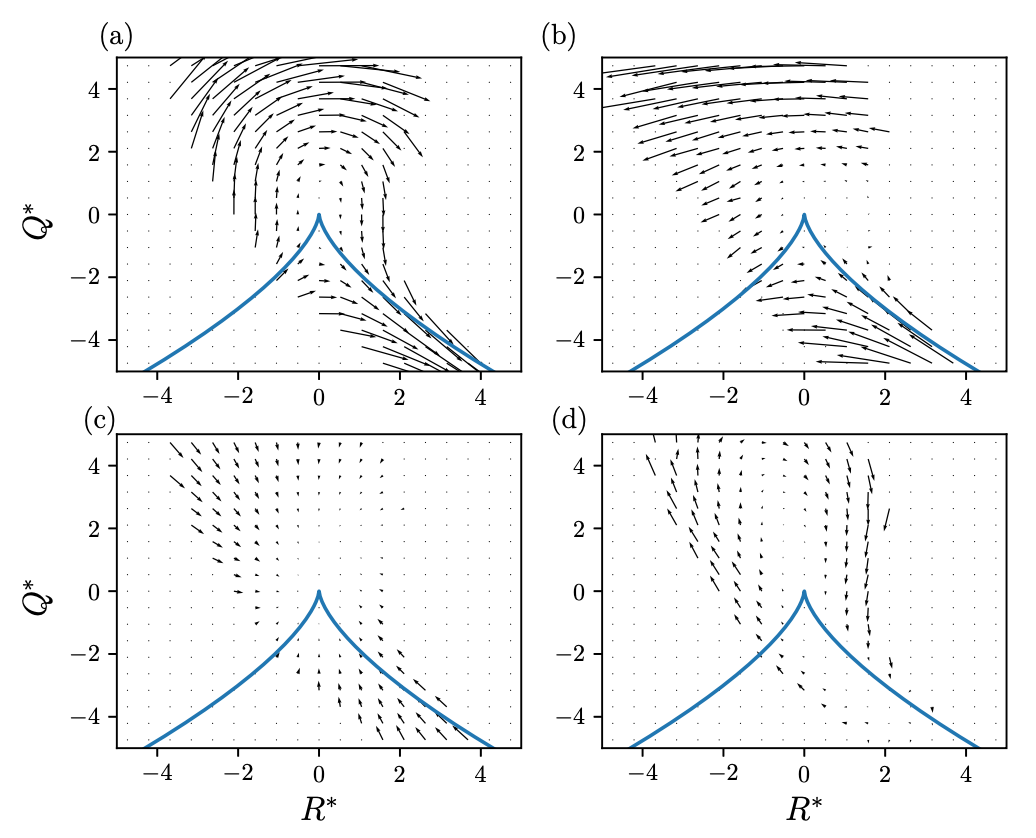
\includegraphics[width=0.75\textwidth]{tian_qr_cmt.png}
%     \caption{The ground truth conditional mean tangents (CMTs) in the $Q\text{-}R$ phase plane arising from (a) Restricted Euler (b) deviatoric pressure Hessian (c) viscous (d) sum of all terms. Taken from Tian et.al, \color{red}{TODO generate this figure.}}
%     \label{fig:gt_qr_cmt}
% \end{figure}
%\subsubsection{Lagrangian Deformation Models}
%Utilizing Lagrangian deformation was first proposed by Chertkov et.al in the Tetrad model\cite{chertkov1999}, which opposed the finite-time singularity by measuring deformation of the tetrad and opposing extreme values. This was interpreted and - using a short-history approximation - adapted into the recent fluid deformation approximation \cite{chevillard2006lagrangian}.
Further development of this idea enriched the upstream initial condition to a Gaussian field approximation.

Johnson and Meneveau \cite{johnson2016} introduced the recent deformation of Gaussian fields (RDGF) model following a long line of postulating that the deviatoric part of the pressure Hessian could be locally modeled using information of the time history of the deformation tensor \cite{chertkov1999},\cite{chevillard2006lagrangian},\cite{chevillard2008modeling}. 

Johnson and Meneveau \cite{johnson2016} introduced the recent deformation of Gaussian fields (RDGF) model, following this line of postulation, and enriching the upstream condition via fitting coefficients of a tensor expansion introduced originally by Pope\cite{pope1975more}. The tensor expansion is treated in detail in section \ref{sec:tbnn}.
%Chertkov et.al's Tetrad Model \cite{chertkov1999}, attempted to capture this deformation directly by following a small fluid element approximated by four Lagrangian particles, initialized in an isotropic configuration. This model avoided the finite time singularity resulting from using only the restricted Euler term\cite{cantwell1992}. Attempts to fuse this low-dimensional model of a fluid element with data-driven methods for prediction of the coarse-grained VGT are ongoing \cite{hyett2021machine},\cite{hyett2020machine}. Chevillard \& Meneveau used the same isotropic Lagrangian upstream condition as in the Tetrad Model when developing their Recent Fluid Deformation (RFD) model. Most recently, Johnson \& Meneveau enriched the approximation of the upstream condition to that of a Gaussian field using high fidelity direct numerical simulation (DNS) data\cite{wan2016johns}.

RDGF models the conditional average of the (full) pressure Hessian tensor as:
\begin{equation}
    \hat{P}_{ij} = \frac{\partial y_k}{\partial x_i} \frac{\partial^2 p}{\partial y_k\partial y_l} \frac{\partial y_l}{\partial x_j} = D^{-1}_{ki} \tilde{P}_{kl} D^{-1}_{lj},
\end{equation}
where $\tilde{P}$ is the pressure Hessian tensor/matrix evaluated along the Lagrangian trajectory upstream in time. The deformation tensor, defined as a sensitivity  of a particle observed at the position $x$ at the moment of time $t$ to its initial position $y$ at the previous moment of time,
\begin{equation}
    D_{ij} = \frac{\partial x_i}{\partial y_j},
\end{equation}
evolves according to 
\begin{equation}\label{eq:Deformation-tensor}
    \frac{d D_{ij}}{dt} = A_{ik} D_{kj}, \quad \text{ with }  D_{ij}(0) = \delta_{ij},
\end{equation}
assuming isotropic initial condition (without loss of generality for sufficiently far removed upstream times). Solution of Eq.~(\ref{eq:Deformation-tensor}) is defined via the time-ordered exponential
\begin{equation} \label{eq:defTensor}
    D(t) = \text{Texp}\left(\int\limits_0^t dt' A(t')\right) = \lim_{N\to \infty} \prod_{i = 0}^N \left( e^{A(t_i)\Delta t} \right),
\end{equation}
where %the product is the left product, and 
$t_i=i \Delta t$ and $\Delta t= t/N$. %t_0 = 0, t_N=t$ and $\Delta t=$. 
If we take $N=1$ and set $\Delta t$ to be the smallest temporal scale of turbulence (also called the Kolmogorov, or viscous scale) we arrive at %the leading order term, we get 
the RDGF approximation for the deformation tensor
\begin{equation}
    \hat{D}(x,t) = \exp\left( A(x,t) \Delta t \right) \approx D(\Delta t).
\end{equation}

All that is left is to determine the upstream pressure Hessian $\tilde P$. The RDGF model uses a Gaussian field closure for $\tilde P$,

\begin{equation} \label{eq:rdgf_upstream}
    \hat{\tilde{P}}_{ij} = \frac{1}{3} \tilde{P}_{kk} \delta_{ij} + \langle \tilde{P}^{(d)}_{ij} | A 
    \rangle_{\text{Gaussian}}
\end{equation}
where $\langle \tilde{P}^{(d)} | A\rangle_{Gaussian}$ is the mean deviatoric pressure Hessian in a Gaussian field, found by Wilczek \& Meneveau\cite{wilczek2014pressure}. Using the notation of the tensor basis [Eqs.~(\ref{eq:tb_start}-\ref{eq:tb_end})], they found
\begin{equation}
    \langle \tilde{P}^{(d)}_{ij} | A \rangle_{\text{Gaussian}} = \gamma T^{(2)} + \alpha T^{(3)} + \beta T^{(4)}
\end{equation}
with the value of the coefficients found from a mix of theoretical and numerical experiments
\begin{equation} \label{eq:rdgf_coefs}
    \alpha = -\frac{2}{7}, \quad \beta=-\frac{2}{5}, \quad \gamma \approx 0.08.
\end{equation}

Introducing the deformed Gaussian field approximation
\begin{equation}
    \hat{G}_{ij} := \hat{D}_{mi}^{-1}\langle \tilde{P}_{mn}^{(d)} | A \rangle_{\text{Gaussian}} \hat{D}_{nj}^{-1},
\end{equation}
and a short-time approximation to the inverse of the left Cauchy-Green tensor
\begin{equation}
    \hat{C}^{-1}_{ij} = \hat{D}^{-1}_{ki}\hat{D}^{-1}_{kj}
\end{equation}
We enforce the prediction in Eq.~(\ref{eq:rdgf_upstream}) to have the correct trace, and arrive at the following RDGF prediction for the component of the pressure Hessian conditioned to the VGT
\begin{equation}
    \hat{P}_{ij} = 2Q \frac{\hat{C}^{-1}_{ij}}{\hat{C}^{-1}_{kk}} + \hat{G}_{ij} - \frac{\hat{C}^{-1}_{ij}}{\hat{C}^{-1}_{kk}}\hat{G}_{ll}.
\end{equation}


\subsubsection{Tensor Basis Neural Network} \label{sec:tbnn}
Contemporaneous to the development of the RDGF model, work was being done to use tensor expansion approximations to the pressure Hessian. Leveraging previous work from Pope\cite{pope1975more}, Lawson and Dawson fit coefficients to a truncated tensor expansion using DNS data\cite{lawson2015}. Tian et.al enriched this approach by parameterizing the coefficient functions, resulting in a so-called tensor basis neural network\cite{tian2021}.

In the case of incompressible turbulence we can write the formal (nonlocal) solution for the deviatoric pressure Hessian as an integral over the spatial domain\cite{ohkitani1995}
\begin{equation} \label{eq:nonlocal_solution}
    H_{ij}({\bm x}) = \iiint \frac{\delta_{ij} - \hat{r_i}\hat{r_j}}{2\pi r^3}Q({\bm x} + {\bm r})d{\bm r}
\end{equation}
where $Q = \frac{1}{2}\tr(A^2)$, and ${\bm x}\in\mathbb{R}^3$.

Lawson \& Dawson \cite{lawson2015}, proposed a local closure based an expansion of the integral in eq(\ref{eq:nonlocal_solution}); first via a Taylor series expansion in words of the strain and rotation rate tensors,
\begin{equation}
  \hat{H} = \sum_{m,n = 0}^\infty \alpha_{mn}S^mW^n
\end{equation}
\begin{equation}
  S = \frac{1}{2}(A + A^T) \qquad W = \frac{1}{2}(A - A^T)
\end{equation}

Then reduced the infinite sum using Cayley-Hamilton theorem on $A$, and expanded via the tensor basis for traceless, symmetric, rotationally invariant function\cite{zheng1993},\cite{pope1975}
\begin{equation}
  \hat{H} = \sum_{n=1}^{10} g^{(n)}(\lambda_1, \dots, \lambda_5)T^{(n)}
\end{equation}
with $g^{(n)}$ scalar functions of the invariants
\begin{equation}
  \lambda_1 = \tr(S^2) \quad \lambda_2 = \tr(W^2) \quad \lambda_3 = \tr(S^3) \quad \lambda_4 = \tr(W^2S) \quad \lambda_5 = \tr(W^2S^2)
\end{equation}
and the tensor basis given by:
\begin{align} \label{eq:tb_start}
  &T^{(1)} = S &T^{(2)} &= SW-WS\\
  &T^{(3)} = S^2 - \frac{1}{3}I \cdot \tr(S^2) &T^{(4)} &= W^2 - \frac{1}{3}I \cdot \tr(W^2)\\
  &T^{(5)} = WS^2 - S^2W &T^{(6)} &= W^2S + SW^2 - \frac{2}{3}I \cdot \tr(SW^2)\\
  &T^{(7)} = WSW^2-W^2SW &T^{(8)} &= SWS^2 - S^2WS\\
  &T^{(9)} = W^2S^2 + S^2W^2 - \frac{2}{3}I \cdot \tr(S^2W^2) &T^{(10)} &= WS^2W^2 - W^2S^2W \label{eq:tb_end}
\end{align}
This formulation reduces the challenge to finding the functions of known scalars. Lawson and Dawson fit constants to a truncated basis expansion (as did the RDGF model for their upstream condition). Tian et.al enriched this approach by learning the $g^{(n)}$'s as shown in fig(\ref{fig:tbnn_architecture}) and using the entire tensor basis. In particular, this allowed the scalar functions to be nontrivial functions of the invariants.

The TBNN architecture ensures the output tensor $\hat{H}$ is symmetric, traceless, and the network itself is rotationally and Galilean invariant. A technical note, since we are using the $L_2$ loss, $\hat{H}$ is only an approximation to the mean deviatoric pressure Hessian if the statistics of the pressure Hessian are normal. As we expect turbulent statistics to be non-Gaussian, the choice of loss is driven more by mathematical convenience. 

\begin{figure}
    \centering
    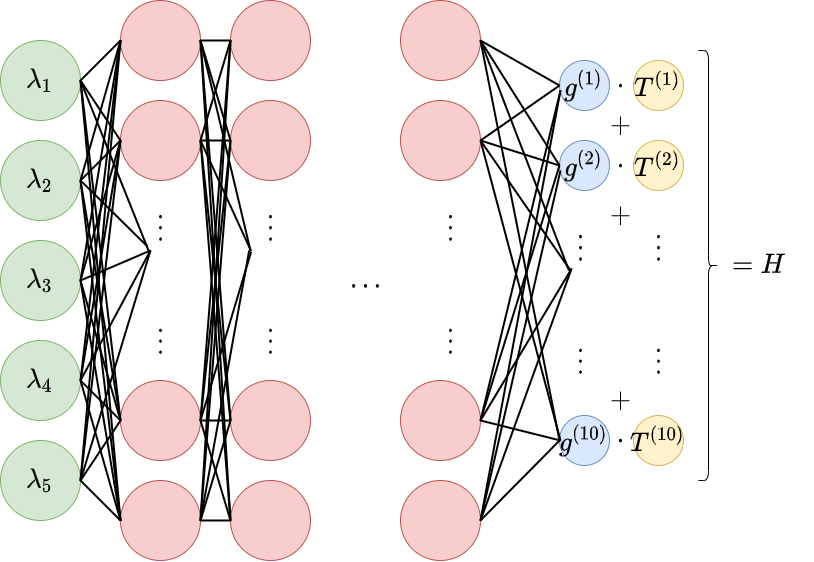
\includegraphics[width=0.5\linewidth]{tbnn.png}
    \caption{The architecture of the TBNN. The invariants and tensor basis elements are calculated from each sample of the VGT, the invariants are then used as input to a fully connected network, and the resulting $g^{(i)}$ multiply the corresponding tensor basis elements $T^{(i)}$, before summing into the prediction $\hat{H}$}
    \label{fig:tbnn_architecture}
\end{figure}

Tian et.al \cite{tian2021} showed ability to train the network, and demonstrated state-of-the-art performance on a variety of relevant physical metrics: eigenvector alignments, $Q\text{-}R$ conditional mean tangents (CMTs), and \textit{a posteriori} tests evolving an initially Gaussian field to fully developed turbulence as evidenced by characteristic teardrop-shaped $Q\text{-}R$ probability distributions (PDFs).

% \begin{figure}
%     \centering
%     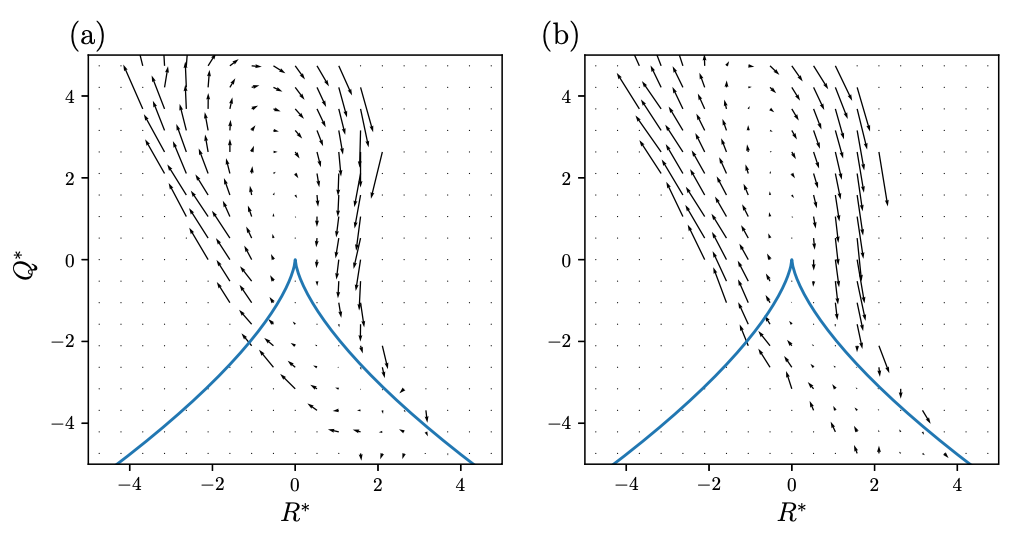
\includegraphics[width=0.85\linewidth]{tian_tbnn_qrcmt.png}
%     \caption{Results from Tian et.al\cite{tian2021} showing $Q\text{-}R$ CMTs from (a) DNS data and (b) trained TBNN}
%     \label{fig:tian_qrcmt}
% \end{figure}



\section{Methodology} \label{sec:methods}
%\subsection{Proposed Models}
Our approach biases the statistics of the conditional deviatoric pressure Hessian using the history of the VGT (as in the RDGF, RFD, and Tetrad models), while avoiding postulating the exact functional form; instead allowing it to be data-driven using PIML (as in TBNN model).

We do this by augmenting the inputs to the feed-forward portion of the TBNN, the idea being to bias the statistics of the invariants, while believing that the tensors derived from the local-in-time VGT are sufficient to span the function space.

    % \item \textbf{RDGF with TBNN output as upstream condition}
    
    % The most logical next step in this progression of deformation models is to enrich the RDGF model using the output of the TBNN. That is, eq(\ref{eq:rdgf_upstream}) becomes
    % \begin{equation} \label{eq:tbnn_rdgf_upstream}
    %     \langle \tilde{P}_{ij} | A \rangle \approx \frac{1}{3} \langle \tilde{P}_{kk} | A \rangle \delta_{ij} + \sum_{n=1}^{10} g_\theta^{(n)}(\lambda_1, \dots, \lambda_5)T^{(n)}
    % \end{equation}
    
    % We believe this has the potential to enrich both models, as Tian et.al, found the different values of parameters in eq(\ref{eq:rdgf_coefs}), and importantly has access to distributions of those parameters. Further, the un-truncated tensor basis has the ability to better represent strongly intermittent conditions. On the other hand, the RDGF model ties this prediction to the local fluid deformation, incorporating temporal information to the local-in-time TBNN.
\subsection{Temporal Convolution}
Motivated by the deformation tensor in eq(\ref{eq:defTensor})
\begin{equation}
  D(t) = \text{Texp}\left(\int\limits_0^t dt' A(t')\right) = \lim_{N\to \infty} \prod_{i = 0}^N \left( e^{A(t_i)\Delta t} \right),
\end{equation}
Each term on the right-hand side of eq(\ref{eq:defTensor}) can be expanded to
\begin{equation}
  e^{A_m \Delta t} = I + \sum_{i=0}^N \frac{1}{i!} \left( \Delta t A_m \right)^i = I + \Delta t A_m+ \bigO(\Delta t^2)
\end{equation}
So that, taking the leading order in $\Delta t$, we obtain the first-order approximation of the deformation tensor
\begin{equation}
  D = I + \Delta t \sum_{n=N}^0 A_n + \bigO(\Delta t^2)
\end{equation}

Therefore, the simplest of our proposed models augments the set of invariants using a learned temporal convolution
\begin{equation} \label{eq:tc_pred}
  \hat{H} = \sum_{n=1}^{10} g_\theta^{(n)}(\lambda_1, \dots, \lambda_5, C)T^{(n)}
\end{equation}
with
\begin{equation}
    C(t) = \sum_{t_f}^{t_f-\Delta t \cdot n} \zeta_n A_n
\end{equation}
where the scalar $\zeta_n$ are learned simultaneously with the parameterization of the scalar $g$ functions.

This model avoids prejudicing the prediction with a specific phenomenological theory of history importance, at the cost of increased computational overhead (namely storing history for each VGT). However, because of the simple structure, the learned $\zeta$'s may inform a temporal correlation in the VGT that is useful in the prediction of the deviatoric pressure Hessian. An extreme case of very short time correlations would reinforce the hypothesis presented in RDGF, while longer temporal correlations would support longer memory approaches e.g., \cite{tian2021_MZ}.

\subsection{Time-Ordered Exponential}
Further, we may hypothesize the exact form of history, replacing $C$ in Eq.~(\ref{eq:tc_pred}) by the true time-ordered exponential 
\begin{equation}
    W(t) = \text{Texp}\left(\int\limits_0^t dt' A(t')\right)
\end{equation}

\subsection{Ground Truth Data \& Training}
Our data is DNS of forced isotropic turbulence with $Re \approx 240$. Eularian data is generated, random points are sampled, VGT and pressure Hessian are constructed at these points using interpolation, and Lagrangian trajectories of these quantities are advanced using the Eularian velocity fields. We have 122k samples, each advanced for 1000 timesteps with $\Delta t = 3e\text{-}4$, representing approximately an inertial eddy turnover time. For each sample and each timestep, we have measured VGT, PH, and viscous terms. We use single timesteps, aggregated over Lagrangian paths separated in time by half an eddy turnover time, as labeled data. As observed by Parashar et.al \cite{parashar2020modeling}, the behavior and training of the TBNN is sensitive to choice of normalization. We follow Tian et.al choosing the physically inspired normalization by Kolmogorov timescale to normalize our input data (and thus the tensor basis itself)
\begin{equation}
  \tau = \frac{1}{\langle \norm{S_{ij}}_2^2 \rangle}
\end{equation}
However, recent work suggests this may be an additional hyperparameter to consider\cite{hyett2022applicability}.

We use a network architecture following Tian et.al's suggestion in their TBNN work\cite{tian2021}, refined using a hyperparameter search\cite{chollet2015keras} across network sizes and shapes, learning rates, and minibatch sizes for each augmentation to the TBNN. The network is trained to minimize the $L_2$ error between the ground truth and predicted pressure Hessian. That is, the optimal parameters are the solution to the optimization
\begin{equation}
  \min_\theta \norm{H - \hat{H}}_2^2
\end{equation}

% \subsubsection{Cramer Functions of Strain Rate Eigenvalues}
% Coarsely stated, the Cramer function (also more generally called the rate function) determines how quickly large deviations from a mean diminish. If we believe in the ability to close the equations for the deviatoric pressure Hessian locally, it is apparent that there must exist a relation between temporal correlations of the strain-rate tensor, and temporal correlations of the deviatoric pressure Hessian.

% \subsubsection{Gaussian Upstream Condition}
% The Gaussian upstream condition present in RDGF is convenient, but for short deformation time is known to be inaccurate. Via analysis of Lagrangian data, we can evaluate how long the deformation time must be to transform the Gaussian upstream condition to a distribution representative of fully developed turbulence. In particular, we can evaluate
% \begin{equation}
%     \min_{\Delta t} \ \norm{P^{(d)}_{gt} - P'^{(d)}_{\text{Gaussian}}(\Delta t)}
% \end{equation}
% where $P'^{(d)}_{\text{Gaussian}}(\Delta t)$ is the true deformation of the Gaussian upstream condition, by the ground truth VGT over a time $\Delta t$.



\section{Results} \label{sec:results}
To evaluate performance of the models, we rely initially on validation loss values as a coarse measure of out-of-testset performance; historically consulted $Q\text{-}R$ phase plane conditional mean tangents (CMTs) as a sanity check; then pressure Hessian eigenvector alignment PDFs as a richer measure of meaningful performance; and finally \textit{a posteriori} tests of $Q\text{-}R$ phase plane PDFs and VGT component PDFs. Comparison of minimum validation loss values tend to indicate general performance across this set of measures, while the remaining measures are in order of increasing physical significance.





\begin{figure}
  \centering
  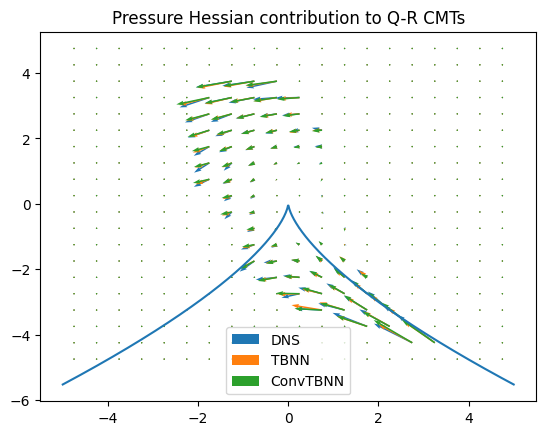
\includegraphics[width=0.5\textwidth]{qr_cmt.png}
  \caption{Qualitatively, the $Q\text{-}R$ conditional mean tangents match the performance of the TBNN}
\end{figure}

\begin{figure}
  \centering
  
\includegraphics[width=0.5\textwidth]{eigenvector_alignment.png}
  \caption{The ConvTBNN outperforms the TBNN in pressure Hessian eigenvector alignment PDF}
\end{figure}

\begin{figure}
  \centering
  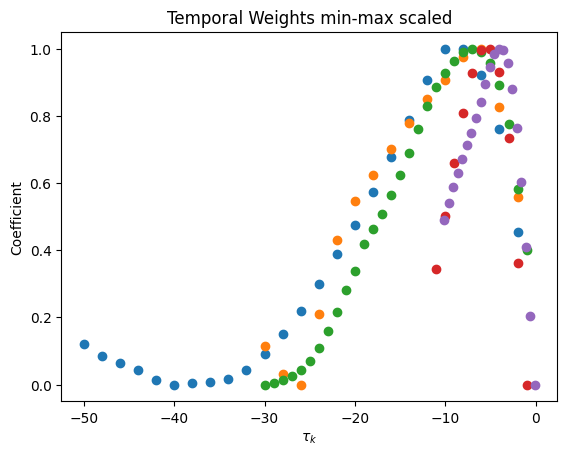
\includegraphics[width=0.5\textwidth]{temporal_conv_kernels_minmax.png}
  \caption{Note 3 items: 1) The convolution weights are small in far history, and for short kernels no flat tails are observed; 2) Weights are small for very recent history; 3) Weights in some importance region increase monotonically.}
\end{figure}


% \subsection{TBNN reproduction}
% After implementing this network architecture and finding the hyperparameters above, the results in figure(\ref{fig:tbnn_reproduction_results}) were found. These results agree well with the original paper, and suggest the hyperparameter choices were accurate.

% \begin{figure}
%     \centering
%     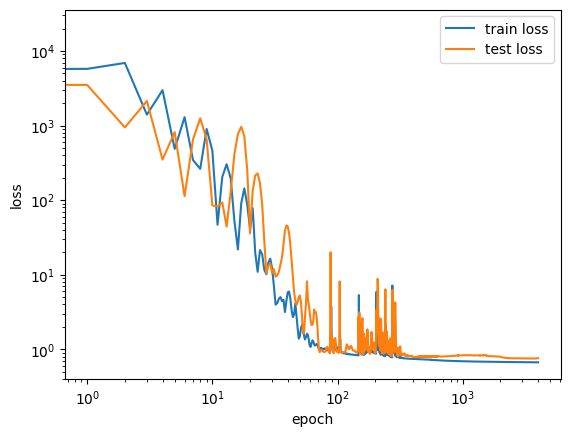
\includegraphics[width=0.5\textwidth]{trained_tbnn_loss.png}%
%     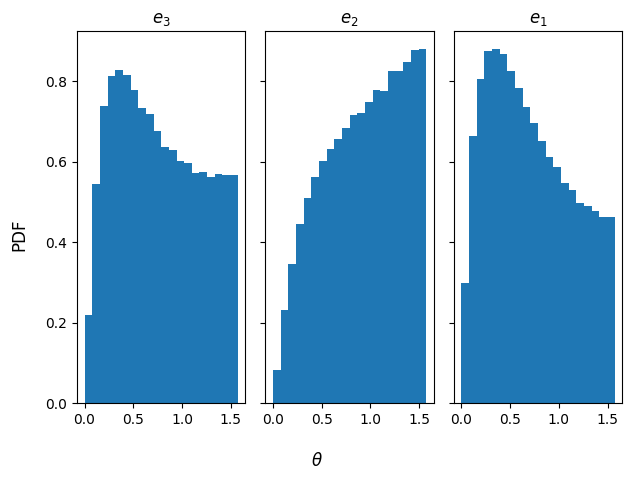
\includegraphics[width=0.5\textwidth]{tbnn_ph_eig_align.png}
%     \caption{(left) Loss as a function of epoch for the TBNN, (right) PDFs of eigenvalue alignment for the pressure hessian, sorted from smallest to largest eigenvalue left to right. These plots agree well with results from Tian et.al's paper, suggesting the implementation is correct.}
%     \label{fig:tbnn_reproduction_results}
% \end{figure}

% \begin{figure}
%     \centering
%     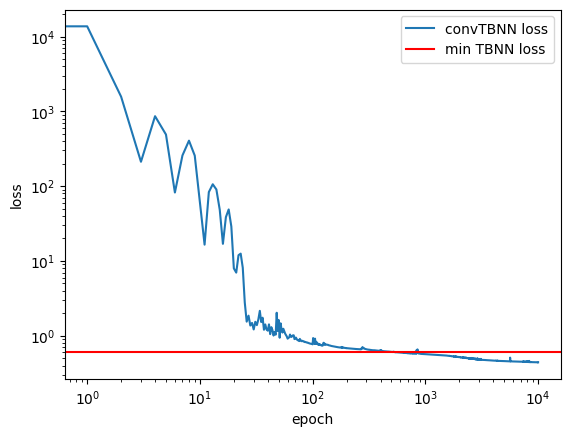
\includegraphics[width=0.5\textwidth]{conv_tbnn_loss.png}%
%     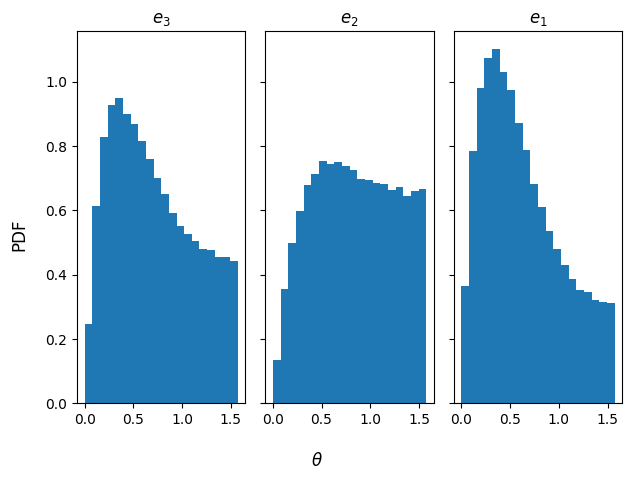
\includegraphics[width=0.5\textwidth]{conv_tbnn_ph_eig_align.png}
%     \caption{Preliminary results of training the convTBNN. (Left) shows the loss vs epoch, with the minimum loss obtained by the unmodified TBNN marked in horizontal red, and the convTBNN in blue. (Right) shows the alignment PDFs of eigenvectors of the PH. Here $e_1$ corresponds to the eigenvector with the greatest associated eigenvalue. Note that compared to fig(\ref{fig:tbnn_reproduction_results}), all alignment PDFs are better, shifting significant density from the misaligned (larger $\theta$) to aligned.}
%     \label{fig:conv_tbnn_results}
% \end{figure}

% \subsection{Temporal Convolution TBNN}
% Preliminary results suggest that the additional historical information of the VGT is in fact useful for the prediction of the PH. In figure(\ref{fig:conv_tbnn_results}), results of training the temporal convolution TBNN (convTBNN) are shown, improving both in the loss and eigenvector alignment metrics.

% \begin{figure}
%     \centering
%     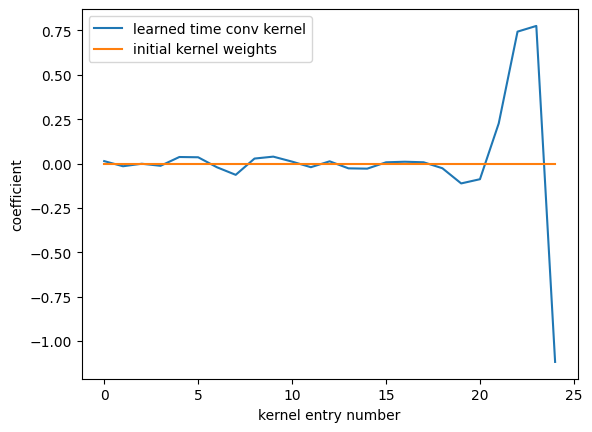
\includegraphics[width=0.5\textwidth]{temporal_conv_kernel.png}
%     \caption{The weights of the learned temporal convolution kernel. This may act as a stand-in for a measure of significance for VGT history as it relates to the prediction of the PH. If these results hold across many trainings, it would suggest that only "recent" history is informative in prediction of the PH.}
%     \label{fig:conv_kernel}
% \end{figure}
% An interesting aspect of the convTBNN is the ability to inspect the kernel length - loosely the length over which the network found it useful to set weights away from zero. Figure(\ref{fig:conv_kernel}) displays the weights as a function of kernel entry number. The sampling in time occurs every $20\Delta t$, where $\Delta t = 3e-4$ and the Kolmogorov timescale is $\tau \approx 3e-3$, so that the sampling occurs about every $2\tau$. We see that only the last three weights are nonzero, suggesting that a history of about $6\tau$ is useful in prediction.

\section{Conclusion} \label{sec:conclusion}
\input{conclusion.tex}

% \section{Appendix}
% \subsection{Interpretability}
Previous work by the authors \cite{hyett2022applicability} suggested there may be a latent space in the invariants when predicting the PH using the TBNN. The existence of a latent space could be important to the ability to interpret the results, e.g. searching for a functional form or providing physical insight; or if we believe in the statistical independence of the input (in our case there are many reasons to) it suggests the network struggles to exploit the additional information. In the case of \cite{hyett2022applicability} it seems to be the latter.

The proposed latent space is indeed persistent when training the network having normalized the PH using $\tau^2$, in particular, the latent space claimed consists only of the low-order invariants. The hypothesis by the author was that the latent space emerged as a numerical artifact of strong normalization of the high-order invariants ($\lambda_{3,4} \to \tau^3 \lambda_{3,4}$, and $\lambda_5 \to \tau^4 \lambda_5$). But as we show in figure(\ref{fig:dg}), there exists leading-order sensitivity to $\lambda_5$ (and not insignficant sensitivity to $\lambda_{3,4}$) when the PH is \textit{not} normalized. This may indicate that the low-order latent space was a numerical artifact resulting from very small weights in the \textit{output layer}, combined with strong normalization of high-order invariants.

\begin{figure}
    \centering
    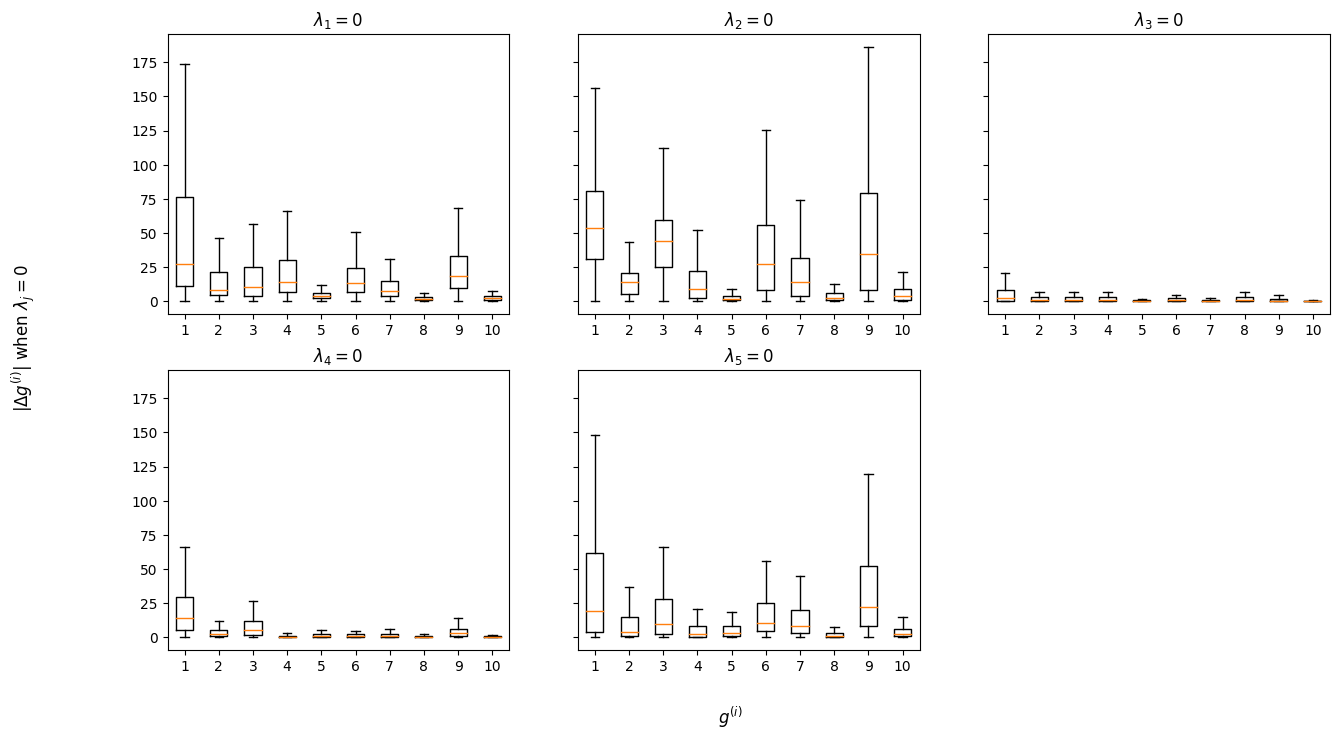
\includegraphics[width=\textwidth]{dg.png}
    \caption{Distributions of sensitivity of $g^{(i)}$ to variability of $\lambda_j$. Previous work performed suggested that $\lambda_{3-5}$ were unimportant to the prediction using the TBNN. This result was predicated upon the normalization of the PH using $\tau^2$. While our plot reinforces that $\lambda_{3,4}$ do provide an order of magnitude smaller correction, the sensitivity of the network to $\lambda_5$ is of the same order of magnitude as that to $\lambda_{1,2}$. This suggests that by \textit{not} normalizing the PH, we are able to exploit additional information in the invariants.}
    \label{fig:dg}
\end{figure}

To explore this question further, we applied an autoencoder to the set of invariants, as well as calculated the mutual information between the invariants.

The mutual information calculation, shown in table(\ref{tab:mutualInformation}), indicates that while the invariants are not strictly independent, they are also far from highly correlated. The maximum value - biased away from the ideal value of $10$ here by the k-nearest neighbors algorithm with $k=5$, detailed in \cite{ross2014mutual}.
\begin{table}
\centering
\begin{tabular}{|c|c|c|c|c|c|}
  \hline
  $I(\lambda_i, \lambda_j)$ & $\lambda_1$ & $\lambda_2$ & $\lambda_3$ & $\lambda_4$ & $\lambda_5$\\
  \hline
  $\lambda_1$ & & 0.26350727 & 1.40593169 & 0.40473788 & 0.72127464\\
  \hline
  $\lambda_2$ & & & 0.1968969 &  0.80102301 & 0.95679744\\
  \hline
  $\lambda_3$ &  &  & & 0.43549834 & 0.49519878\\
  \hline
  $\lambda_4$ & & & & & 0.83990126\\
  \hline
  $\lambda_5$ & & & & & \\
  \hline
\end{tabular}
  \caption{A scaled mutual information $I(\lambda_i, \lambda_j)$, between invariants. Note the maximum value is near $10$, the method used here introduces a bias however, namely via k-nearest neighbors with $k=5$, as discussed in \cite{ross2014mutual}}
    \label{tab:mutualInformation}
\end{table} 

\begin{figure}
    \centering
    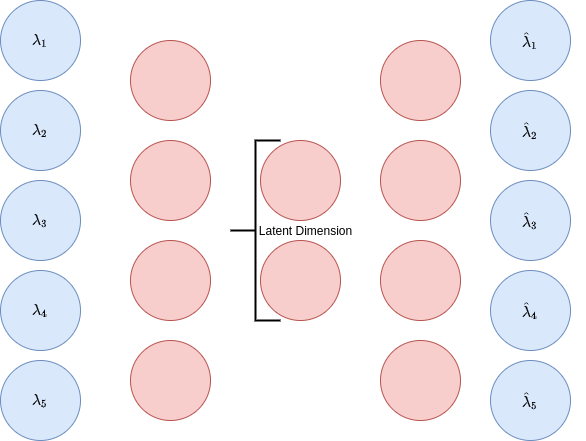
\includegraphics[width=0.5\textwidth]{aeStructure.png}
    \caption{Autoencoder structure applied to the invariant input data.}
    \label{fig:aeStructure}
\end{figure}

The autoencoder structure is a fully connected, feed forward neural network, 
\begin{equation}
    AE_\theta: \R^5 \to \R^5 \text{ via } \R^5 \to \R^4 \to \R^h \to \R^4 \to \R^5
\end{equation}
where $h$ is the imposed latent dimension, illustrated in fig[\ref{fig:aeStructure}]. The nonlinear activation functions of $AE_\theta$ are the so-called "leaky-relu". We implement the "robust max-min" normalization, relying on the interquartile distance - namely, letting $Q_1, Q_3$ be the first and third quartiles, we normalize our invariants as
\begin{equation}
    \Tilde{\lambda_i} = \frac{\lambda - Q_1}{Q_3 - Q_1}
\end{equation}
This is intentionally different than the normalization used in the TBNN, as normalizing via timescale and optimizing using the mean-squared-error gives a very strong preference towards reconstructing only the low-order invariants. The robust max-min normalization is an attempt to set each on an equal footing, but itself is subject to biases introduced by differences in distribution shapes.

We use the ADAM optimizer with learning rate $\eta = 1e-3$, partitioning the dataset of 100k samples into 75\% training, 25\% test. The results are shown in fig[\ref{fig:aeLoss}] and may suggest a small reduction in dimension (i.e., $5\to 3$). These results match the leading order contributions to the sensitivities of the $g^{(i)}$ as shown in fig(\ref{fig:dg}), but we caution this suggestion as the low-order basis elements are still significantly influenced.
\begin{figure}
    \centering
    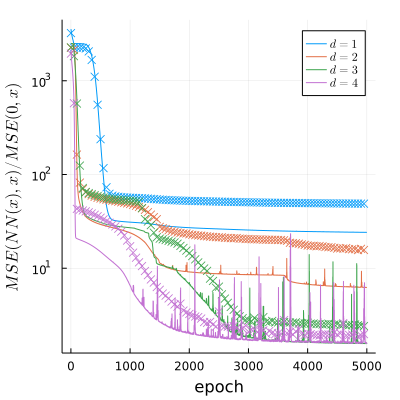
\includegraphics[width=\textwidth]{aeInvariants.png}
    \caption{Autoencoder applied to the invariant input data, in an attempt for a nonlinear projection onto a latent space. (Left) shows the evolution of the loss according to the imposed latent dimension, where 'x's mark test loss, while solid lines mark training loss. (Right) shows the minimum loss as a function of latent dimension. Notice the two jumps at $h = 2$ and $h=3$ - suggesting a sequence of increasing fidelity.}
    \label{fig:aeLoss}
\end{figure}


% \nocite{*}
\bibliographystyle{plain}
\bibliography{refs}

\end{document}